% Classe de documento.
\documentclass[a4paper,12pt,openright,titlepage,oneside]{book}

%Define regra de gramática para separar síbalas {babel}
%e altera os títulos (como chapters, sections, references) para português
\usepackage[brazil]{babel}

% Define uso de caracteres acentuados no PDF gerado
% e permite copiar corretamente o texto do PDF.
\usepackage[T1]{fontenc}
\usepackage[utf8]{inputenc}

% Outros pacotes utilizados.
\usepackage{subfigure}

% Adição do pacote do template da UnB.
\usepackage{styles/template-FT-UnB/ft2unb}

\DeclareGraphicsExtensions{.jpg,.pdf,.mps,.png,.gif, .eps}
\graphicspath{images} %define diretório de imagens

%Arquivo com lista com hifenização correta de algumas palavras.
%Defina novas palavras no arquivo a medida que verificar que a hifenização automática
%etá errada para tais palavras.
\input{styles/hifenizacao}

% ALTERE OS VALORES DENTRO DAS CHAVES DOS COMANDOS NESTA SEÇÃO PARA INCLUIR OS SEUS DADOS E DADOS DA SUA
% DISSERTAÇÃO DE MESTRADO OU TESE DE DOUTORADO
% -----------------------------------------------------------------------------------------------------

%\onehalfspacing
\title{Previsão de insuficiência cardíaca com aprendizado de máquina em um website}
\author{André Filipe Caldas Laranjeira}
\date{2021-05-19} %data da defesa
\coverbackgroundimg{images/capa_fundo}

\grau{Bacharel}
\area{Engenharia da computação} %Nome do curso
\departamento{Ciência da computação} %Nome do departamento
\faculdade{INSTITUTO DE CIÊNCIAS EXATAS} %Nome da faculdade/instituto
\siglafaculdade{IE} %Sigla da faculdade/instituto
\siglaarea{CIC} %Sigla do departamento
\tipodemonografia{Monografia} %Dissertação ou Tese
\programa{Bacharelado} %Mestrado ou Doutorado
\autorendereco{Área Octogonal Sul 2, Bloco G, Apartamento 601; Octogonal, Brasília} %Endereço do autor da dissertação/tese
\totalpgs{32} %total de páginas atualmente na sua dissertação
\dia{19} %dia da defesa
\mes{Maio} %mês da defesa
\ano{2021} %ano da defesa
\numpublicacao{xxx/AAAA} %número da publicação (após a defesa, tal número deve ser obtido na secretaria)

%PPGENE.DM  = Programa de Pós Graduação em ENgenharia Elétrica.Dissertação de Mestrado
%PPGENE.TD  = Programa de Pós Graduação em ENgenharia Elétrica.Tese de Doutorado
\siglapublicacao{?}

\titulolinhai{Previsão de insuficiência cardíaca}
\titulolinhaii{com aprendizado de máquina}
\titulolinhaiii{em um website}

\autori{André Filipe Caldas Laranjeira}
%Caso seu nome não caiba em uma única linha, divida ele nos comandos abaixo
%\autorii{}
%\autoriii{}

\membrodabancai{Prof. Dr. Alexandre Ricardo Soares Romariz, ENE/UnB}
\membrodabancaifuncao{Orientador}
\membrodabancaii{Prof. Dr. Adson Ferreira da Rocha, ENE/UnB}
\membrodabancaiifuncao{Examinador interno}
\membrodabancaiii{Prof. Dr. Li Weigang, CIC/UnB}
\membrodabancaiiifuncao{Examinador interno}
% -----------------------------------------------------------------------------------------------------

%line-numbers, inputencoding=utf8/latin1
%Define o estilo para listagens de código fonte
\lstset{
  numbers=left, %numeração de linhas à esquerda
  stepnumber=1,
  firstnumber=1,
  numberstyle=\tiny,
  extendedchars=true,
  frame=none,
  basicstyle=\footnotesize,
  stringstyle=\ttfamily,
  showstringspaces=false,
  %language=Java, %deve ser definida na inclusão de cada trecho de código, pois podem existir linguagens diferentes em exemplos diferentes
  breaklines=true,
  breakautoindent=true,
  %estilos de comentário de uma e várias linhas
  morecomment=[l]{--}, morecomment=[s]{/*}{*/}, morecomment=[s]{<!--}{-->}, morecomment=[s]{--[[}{--]]}
}

% Adição de metadados no PDF (propriedades do documento PDF)
\makeatletter
	 \hypersetup{
		 pdftoolbar=true,        % show Acrobat’s toolbar?
		 pdfmenubar=true,        % show Acrobat’s menu?
		 pdffitwindow=false,     % window fit to page when opened
		 pdfstartview={FitH},    % fits the width of the page to the window
		 pdftitle={\@title},
		 pdfauthor={\@author},
		 pdfsubject={\tipodemonografianome \ de\ \programastr \ em\ \areastr},   % subject of the document
		 pdfcreationdate={\pdfdate}
	 }
\makeatother


\makeindex
\makenomenclature %Necessário para gerar lista de siglas


\begin{document}

	\pdfbookmark[0]{Agradecimentos}{agradecimentos}
	\include{sections/agradecimentos}
	Este trabalho consiste em um estudo comparativo entre modelos de aprendizado de máquina do tipo perceptron multicamada e floresta aleatória treinados para a previsão de insuficiência cardíaca e em um website auxiliar para utilização do melhor modelo. Sua importância se dá pela implementação de uma aplicação prática, na forma de um website, para modelos de aprendizado de máquina. A avaliação dos modelos de treinamento se baseou na melhor média de acurácia de previsão envolvendo 20 subconjuntos de validação e 100 subconjuntos de teste. Ao total 5346 modelos de treinamento foram avaliados e o modelo mais bem classificado obteve uma média de acurácia comparável àquela do artigo de referência utilizado. A implementação do website auxiliar também obteve êxito ao simplificar o acesso ao melhor modelo de previsão. Para trabalho futuros, planeja-se a avaliação de mais tipos de modelo de aprendizado de máquina e suas combinações de hiperparâmetros, a criação de um aplicativo móvel e a realização de testes do melhor modelo com pacientes contemporâneos.


	\pdfbookmark[0]{Sumário}{sumario}
	\sumario

	\pdfbookmark[0]{Lista de Figuras}{listafiguras}
	\listadefiguras

	\pdfbookmark[0]{Lista de Tabelas}{listatabelas}
	\listadetabelas

	\pdfbookmark[0]{Lista de Códigos Fonte}{listacodigosfonte}
	\listadecodigosfonte

	\renewcommand{\nomname}{LISTA DE TERMOS E SIGLAS} %Define um caption à lista de siglas
	%Inclui a lista de siglas
	\pdfbookmark[0]{Lista de Termos e Siglas}{nomenclatura}
	\printnomenclature[2.5cm]

	\mainmatter %Inicia a numeracao normal cardinal
	\setcounter{page}{1} \pagenumbering{arabic} \pagestyle{plain}

	\chapter{Introdução} \label{chap:introducao}

Este trabalho realiza um estudo comparativo de modelos de aprendizado de máquina do tipo perceptron multicamada e floresta aleatória treinados com um conjunto de variáveis relacionadas à saúde cardiovascular e geral para realizar uma previsão da sobrevivência à insuficiência cardíaca de um paciente humano antes do final de um período de acompanhamento médico de duração média de 130 dias. Além disso, neste trabalho também foi implementado um website para permitir que o modelo de treinamento com a melhor acurácia de previsão no estudo mencionado possa ser acessado e utilizado de forma simples e direta por um público alvo abrangente.

Com este trabalho, espera-se exemplificar como uma aplicação concreta, mais especificamente um website, pode ser construída ao redor de um estudo de aprendizado de máquina para permitir que um modelo de aprendizado de máquina seja utilizado por profissionais da saúde para fornecer benefícios concretos no atendimento a pacientes.

O trabalho está organizado no formato descrito a seguir. O capítulo \ref{chap:apresentacao_teorica} apresenta ao leitor conceitos teóricos fundamentais para o entendimento deste trabalho. O capítulo \ref{chap:procedimento_adotado} descreve o procedimento adotado pelo autor na realização deste trabalho. O capítulo \ref{chap:resultados} apresenta os resultados obtidos neste trabalho. Por fim, o capítulo \ref{chap:conclusao} apresenta a conclusão deste trabalho e sugere futuras pesquisas a serem realizadas com base neste trabalho.

Todo o código fonte utilizado para este trabalho pode ser encontrado no repositório do \textit{GitHub} para este trabalho\footnote{\url{https://github.com/AndreLaranjeira/ML-HeartFailureSurvival}}.

\section{Relevância da temática}

A insuficiência cardíaca é uma condição clínica crônica e progressiva em que o coração não consegue bombear sangue suficiente para todo o corpo resultando em sintomas como fadiga e problemas respiratórios \cite{heart_failure_definition}. Os principais fatores que aumentam o risco de desenvolvimento de insuficiência cardíaca são doenças arteriais coronarianas, hipertensão, diabetes, obesidade e fumo \cite[p.399]{heart_disease2021}. Além disso, estudos recentes demonstraram que a falta de boas condições físicas nos sistemas cardíaco e respiratório também contribui para o aumento do risco de desenvolvimento de insuficiência cardíaca \cite[p.62]{heart_disease2021}.

A ocorrência de insuficiência cardíaca possui grande relevância nos dias atuais. Segundo a Associação Americana do Coração (AHA)\nomenclature{AHA}{Associação Americana do Coração}, dados coletados entre 2015 e 2018 apontam que 6 milhões de adultos estadunidenses com mais de 20 anos tiveram insuficiência cardíaca \cite[p.8]{heart_disease2021} e que 83.616 estadunidenses vieram a óbito em 2018 por insuficiência cardíaca \cite[p.485]{heart_disease2021}. No Brasil, um estudo publicado em 2019 na revista Acta Fisiátrica \cite{nogueira2019} utilizou dados de 2013 para estimar que 1,7 milhões de brasileiros já tiveram insuficiência cardíaca e outro estudo publicado em 2014 nos Arquivos Brasileiros de Cardiologia \cite{gaui2014} aponta que aproximadamente 27.702 brasileiros vieram a óbito em 2011 por insuficiência cardíaca.

Por fim, devemos salientar o impacto econômico causado por essa condição clínica. De acordo com uma diretriz de insuficiência cardíaca dos Arquivos Brasileiros de Cardiologia \cite{diretriz_insuficiencia_cardiaca_2018}, os gastos globais governamentais e privados com essa condição clínica foram de R\$ 14,5 bilhões apenas em 2015.

O uso de programas de aprendizado de máquina que prevejam a ocorrência de insuficiência cardíaca e a mortalidade por insuficiência cardíaca pode auxiliar na redução do número de pessoas que sejam afligidas e que venham a óbito por essa condição médica, respectivamente. Isso resultaria na diminuição dos recursos monetários despendidos globalmente, direta ou indiretamente, no tratamento da insuficiência cardíaca. Além disso, a saúde geral da população mundial seria beneficiada com a diminuição do número de ocorrências de insuficiência cardíaca.

\section{Literatura existente}

Artigos recentes exploraram vários aspectos sobre como o aprendizado de máquina pode ser utilizado para combater a insuficiência cardíaca. Um artigo escrito por Awan, Sohel e outros revisou estudos existentes acerca das possibilidades de uso de aprendizado de máquina para melhorar os tratamentos e diagnósticos de insuficiência cardíaca e assim diminuir gastos com essa condição médica \cite{awan2018}. Um outro artigo publicado no jornal europeu de insuficiência cardíaca utiliza o aprendizado de máquina para correlacionar pacientes e desenvolver uma nova métrica de risco de óbito por insuficiência cardíaca que obteve mais acurácia que as métricas existentes \cite{adler2020}. Por fim, um outro artigo publicado no jornal da sociedade americana de ecocardiografia propós um programa de aprendizado de máquina para identificar a presença de insuficiência cardíaca com preservação na taxa de ejeção, um tipo específico de insuficiência cardíaca, por meio de imagens ecocardiográficas que mensurem as velocidades miocárdicas em repouso e durante exercício \cite{hfpef2018}.

Dentre a literatura existente, forneceremos destaque especial ao artigo publicado por Chicco e Jurman \cite{chicco2020}. Esse artigo faz uso de um conjunto de dados de pacientes que foram hospitalizados com insuficiência cardíaca \cite{larxel_dataset} disponibilizado em um artigo científico de 2017 \cite{dataset_article}, utilizando esse conjunto de dados tanto para realizar uma análise comparativa da performance obtida na previsão de sobrevivência à insuficiência cardíaca com o uso de difentes modelos de treinamento e variáveis dos pacientes como para identificar quais variáveis do conjunto de dados possuem maior correlação com a ocorrência de óbito por insuficiência cardíaca. Adotamos o artigo publicado por Chicco e Jurman como a principal referência utilizada neste trabalho devido à semelhança dos objetivos propostos para o uso do aprendizado de máquina neste trabalho e no artigo em questão e ao fato de que este trabalho utiliza o mesmo conjunto de dados que o artigo em questão como fonte de experiência do aprendizado de máquina.

	\chapter{Apresentação teórica} \label{chap:apresentacao_teorica}

Neste capítulo, alguns conceitos teóricos são explanados com o intuito de fornecer ao leitor o embasamento teórico necessário para a compreensão completa deste trabalho.

\section{Aprendizado de máquina}

O campo de estudo de aprendizado de máquina é uma vasta área da computação, possuindo várias aplicações, objetos de estudo e focos de pesquisa interdisciplinares. Resumidamente, podemos dizer que essa área estuda como "construir programas de computador que melhoram seu desempenho em alguma tarefa por meio da experiência"\footnote{\cite[p.29]{machine_learning}}. Atualmente, utilizamos o aprendizado de máquina para várias aplicações como algoritmos de recomendações de conteúdo, programas de reconhecimento e classificação de imagens e a realização de análises de risco financeiro.

Para utilizarmos o aprendizado de máquina para resolvermos alguma problema, faz-se necessário definir matematicamente uma tarefa a ser realizada, uma ou mais métricas de desempenho atreladas à realização da tarefa e a fonte de experiência que será utilizada pelo modelo para aprender a realizar a tarefa.\footnote{\cite[p.29]{machine_learning}} Também precisamos escolher um ou mais tipos de modelo de aprendizado de máquina que serão utilizados para aprender a realizar a tarefa com base em um treinamento feito com a fonte de experiência avaliado sob a ótica das métricas de desempenho escolhidas.

\subsection{Especificação de uma tarefa}

Qualquer problema de aprendizado de máquina deve possuir uma tarefa a ser realizada, que representa o objetivo a ser atingido pelo uso de aprendizado de máquina. A especificação dessa tarefa sempre deve possuir o formato de uma função matemática para permitir que um programa de computador consiga aprendê-la. Assim, podemos afirmar que qualquer tarefa de aprendizado de máquina pode ser representada, genericamente, pela função $T : V \rightarrow R$, onde $V$ é um conjunto de variáveis disponibilizado para a realização da tarefa de aprendizado de máquina e $R$ é o resultado esperado da tarefa de aprendizado de máquina.

Para um programa de aprendizado de máquina realizar a tarefa proposta, este deve aprender a função $T$. Entretanto, na grande maioria dos problemas de aprendizado de máquina, a função $T$ não é conhecida e o problema proposto se resume a aproximar uma \textit{descrição operacional} de $T$.\footnote{\cite[p.8]{machine_learning}} Dessa forma, o programa de aprendizado de máquina deve então utilizar o processo de aprendizado com base na fonte de experiência para adquirir uma função $\hat{T}$ que seja uma boa aproximação da função $T$.

Neste trabalho, o problema de previsão de insuficiência cardíaca pode ser descrito como sendo um problema de \textit{classificação binária}, em que a tarefa proposta é representada pela função $P : V_{p} \rightarrow [0, 1]$, onde $V_{p}$ são as variáveis fornecidas que descrevem o paciente e o conjunto imagem $[0, 1]$ representa uma previsão se o paciente irá vir a óbito (1) ou não (0).

\subsection{Fonte de experiência}

Para permitir que um programa de aprendizado de máquina aprenda uma aproximação $\hat{T}$ da função $T$, é necessário a utilização de uma fonte de experiência que forneça, direta ou indiretamente, uma maneira do programa de treinamento inferir o comportamento da função $T$. Essa fonte de experiência pode ser obtida de várias formas, as quais variam consideravelmente dependendo da tarefa em questão e do método de aprendizado almejado para o programa computacional, de forma que o tipo de recurso utilizado como fonte de experiência não apenas é determinante no sucesso ou fracasso do aprendizado, como também define uma categoria de aprendizado que será adotada pelo programa computacional.

O tipo mais comum de fonte de experiência utilizada é um conjunto de dados com exemplos que possuem variáveis e o resultado da aplicação dessas variáveis à função $T$, categoria de aprendizado conhecida como aprendizado supervisionado. Alguns outros tipos de fontes de experiência e suas respectivas categorias de aprendizado incluem: o uso de um conjunto de dados com exemplos com variáveis mas sem nenhum resultado da função $T$, categoria conhecida como aprendizado não supervisionado; o uso de um conjunto de dados com exemplos com variáveis mas nem sempre com o resultado da aplicação dessas variáveis à função $T$, categoria conhecida como aprendizado semi-supervisionado; e uma exploração da função $T$ feita pelo próprio programa computacional com base em uma métrica de recompensa, categoria conhecida como aprendizado por reforço.

Para que a função de aproximação $\hat{T}$ aprendida pelo programa de aprendizado de máquina com base na fonte de experiência utilizada seja uma boa aproximação da função $T$, é necessário que a fonte de experiência utilizada seja uma boa aproximação dos exemplos que o programa de aprendizado de máquina encontrará ao longo de sua avaliação e uso, uma suposição que quase sempre se revela como falsa.\footnote{\cite[p.6]{machine_learning}} Isso pode levar a ocorrência de um fenômeno denominado sobreajuste (ou \textit{overfitting}) no processo de aprendizado do programa computacional. Esse fênomeno ocorre quando o processo de aprendizado é aplicado excessivamente na fonte de experiência utilizada, piorando a aproximação $\hat{T}$ aprendida pelo programa computacional devido às discrepâncias entre os dados englobados na fonte de experiência e os dados englobados em todo o domínio da função $T$.

Neste trabalho, o programa de previsão de insuficiência cardíaca utilizou como fonte de experiência para seu treinamento um conjunto de dados\footnote{\cite{larxel_dataset}} composto de exemplos com variáveis e o resultado da aplicação dessas variáveis à função $T$, tomando parte, assim, na categoria de problemas de aprendizado supervisionado. O capítulo \ref{chap:procedimento_adotado} aborda alguns cuidados utilizados para evitar a ocorrência de sobreajuste no processo de aprendizado.


	\chapter{Procedimento adotado} \label{chap:procedimento_adotado}

Neste capítulo, o procedimento adotado ao longo do trabalho é detalhado com o intuito de permitir ao leitor compreender melhor a lógica por trás de algumas escolhas feitas no decorrer do trabalho e de explorar alguns detalhes importantes da implementação dos módulos de programação.

\section{Conjunto de dados}

Como primeiro passo no processo de aprendizado de máquina, foi necessária a escolha de um conjunto de dados que possibilitasse o treinamento de modelos de aprendizado de máquina para uso em uma aplicação completa em tempo útil para a realização deste trabalho. Tendo isso em mente, a decisão recaiu sobre um conjunto de dados\cite{larxel_dataset} originado de um artigo científico escrito por Chicco e Jurman\cite{chicco2020} voltado para o estudo de aprendizado de máquina para a previsão de ocorrência de insuficiência cardíaca.

O conjunto de dados escolhido contém 299 registros de pacientes, cada um consistindo em 11 variáveis relacionadas à saúde geral e cardíaca de um paciente, 1 variável indicando o tempo de acompanhamento médico do paciente e 1 resultado indicando se o paciente veio a óbito durante o acompanhamento realizado. Dessa forma, trata-se de um conjunto de dados pequeno, de fácil compreensão, que pudesse ser explorado com um certo grau de profundidade em um curto espaço de tempo, e com uma clara utilidade prática de auxiliar a prevenção da ocorrência de insuficiência cardíaca em pacientes com base em uma previsão realizada por meio de aprendizado de máquina. Para fins deste trabalho, apenas 10 das 12 variáveis fornecidas pelo conjunto de dados foram utilizadas.

Além das características úteis do conjunto de dados em si para a realização deste trabalho, o artigo científico que originou o conjunto de dados consiste em um estudo comparativo do desempenho de diferentes tipos de modelos de dados na previsão de insuficiência cardíaca com base no conjunto de dados em si, proporcionando uma referência útil para a realização de escolhas do tipo de modelo de aprendizado de máquina a ser utilizado no conjunto de dados e para a comparação dos resultados atingidos no treinamento de modelos de aprendizado de máquina.

Apesar dessas qualidades, devemos ressaltar que o conjunto de dados escolhido não é sem falhas. A baixa quantidade de registros no conjunto de dados faz com que o treinamento de modelos de aprendizado de máquina seja extremamente suscetível a \textit{overfitting}, resultando em um modelo que não forneça bons resultados em aplicações práticas. Também podemos notar que a baixa quantidade de registros em que o paciente veio a óbito, agravada pelas subdivisões do conjunto de dados em dados de treinamento, de teste e de validação, pode gerar modelos com um viés para previsões positivas, aumentando a probabilidade de que o modelo de aprendizado de máquina gere falsos negativos, em que o sistema não prediz a insuficiência cardíaca e o paciente vem a óbito. A forma como essas limitações da base de dados foram tratadas será descrita posteriormente.

\section{Modelos de treinamento de aprendizado de máquina}

Com a escolha do conjunto de dados feita, o próximo passo seria definir quais tipos de modelos de treinamento de aprendizado de máquina seriam avaliados para uso na aplicação e estabelecer um método específico de avaliação para permitir a comparação entre os diferentes modelos de treinamento e determinar qual deveria ser utilizado na aplicação.

\subsection{Tipos de modelos testados}

Inicialmente, o propósito deste trabalho consistia em avaliar exclusivamente o desempenho de modelos do tipo redes neurais de perceptron multicamada. Entretanto, a leitura da análise realizada e dos resultados obtidos no artigo científico de Chicco e Jurman\cite{chicco2020} que originou o conjunto de dados utilizado\cite{larxel_dataset}, bem como o tempo necessário para o treinamento de um único modelo de perceptron multicamada, levaram a realização de análises adicionais com modelos do tipo floresta aleatória, os quais obtiveram a melhor acurácia de previsão de acordo com os resultados do artigo científico de Chicco e Jurman e podem ser treinados em uma fração do tempo de treinamento de modelos do tipo perceptron multicamada.

\subsection{Método de avaliação dos modelos de treinamento}

Com o intuito de comparar diferentes modelos de treinamento de aprendizado de máquina, um método padrão de avaliação foi adotado com base no método utilizado no artigo científico de Chicco e Jurman\cite{chicco2020}. Esta subseção, com o intuito de justificar algumas das escolhas feitas na montagem do método de avaliação adotado, descreve formalmente tanto o método de avaliação de modelos de treinamento utilizado no artigo científico de Chicco e Jurman, como o método de treinamento utilizado neste trabalho.

\subsubsection{Método de avaliação de modelos de treinamento utilizado no artigo científico}

O artigo científico de Chicco e Jurman em que o conjunto de dados\cite{larxel_dataset} foi primeiramente apresentado e que buscou estudar vários aspectos do aprendizado de máquina aplicado ao conjunto de dados utilizou um método específico para avaliar quais foram os melhores modelos de aprendizado de máquina. Esse método consistiu em dois submétodos diferentes para modelos com otimização de hiper-parâmetros e para modelos sem otimização de hiper-parâmetros.

Para tipos de modelos com otimização de hiper-parâmetros, o conjunto de dados foi dividido em 60\% de dados para treinamento, 20\% de dados para validação e 20\% de dados para teste. Primeiramente, vários modelos com diferentes hiper-parâmetros foram treinados com o subconjunto de dados de treinamento com o intuito de encontrar o conjunto de hiper-parâmetros que gerasse o melhor coeficiente de correlação de Matthews (MCC) relativo à previsão feita sobre o subconjunto de dados de validação. Esse conjunto de hiper-parâmetros então foi utilizado em um novo modelo, treinado com o subconjunto de dados de treinamento, para obter o coeficiente de correlação de Matthews (MCC) relativo à previsão feita sobre o subconjunto de dados de teste. Esse procedimento foi realizado sobre 100 diferentes partições do conjunto de dados, para que a média e mediana dos 100 resultados de coeficiente de correlação de Matthews (MCC) relativos às previsões feitas sobre os subconjuntos de dados de teste com aquele tipo de modelo fossem calculados.

Para tipos de modelos sem otimização de hiper-parâmetros, o conjunto de dados foi dividido em 80\% de dados para treinamento e 20\% de dados para teste. Um modelo foi treinado com o subconjunto de dados de treinamento para obter o coeficiente de correlação de Matthews (MCC) relativo à previsão feita sobre o subconjunto de dados de teste. Esse procedimento foi realizado sobre 100 diferentes partições do conjunto de dados, para que a média e mediana dos 100 resultados de coeficiente de correlação de Matthews (MCC) relativos às previsões feitas sobre os subconjuntos de dados de teste com aquele tipo de modelo fossem calculados.

\subsubsection{Método de avaliação de modelos de treinamento utilizado neste trabalho}

Neste trabalho, o método utilizado para avaliar quais modelos de treinamento obtiveram os melhores resultados baseou-se no método de avaliação utilizado no artigo científico de Chicco e Jurman, mas com algumas alterações.

Em primeiro lugar, 100 inteiros de 32 bits sem sinal foram gerados e armazenados em um arquivo para serem utilizados como sementes na aleatoriedade inerente ao particionamento do conjunto de dados\cite{larxel_dataset}, de forma que todos os modelos agora utilizam as mesmas partições do conjunto de dados para realizarem seu treinamento e obterem seus resultados de validação e teste. Essa mudança foi feita com o intuito de permitir a replicação dos resultados obtidos e proporcionar uma forma mais justa de comparação entre diferentes modelos com diferentes hiper-parâmetros. Além disso, como o tempo de treinamento de alguns modelos pode ser consideravelmente longo, essa técnica permite que a obtenção de um resultado de validação ou teste para um mesmo modelo seja dividida em mais de uma execução, dado que um subconjunto de dados de validação e teste é fixo para uma dada semente escolhida.

Em segundo lugar, a otimização de hiper-parâmetros não pôde ser feita da mesma forma que o artigo científico de Chicco e Jurman, pois a quantidade de combinações de hiper-parâmetros existente não permitiria que todas as variações de hiper-parâmetros fossem testadas para um dado modelo e uma dada partição do conjunto de dados. Dessa forma, decidiu-se que a única otimização de hiper-parâmetros feita seria na quantidade de épocas de treinamento para modelos do tipo perceptron multicamada. O número de épocas escolhido para treinamento na obtenção dos resultados de teste será equivalente à época em que o modelo teve a menor perda nos dados de validação (abordagem conhecida como \textit{early stopping}). Para os demais parâmetros, decidiu-se adotar o seguinte procedimento: várias variações de hiper-parâmetros seriam utilizadas para se obter o resultado de predição sobre os subconjuntos de validação do primeiro quinto das partições de dados disponíveis (20), e as combinações de hiper-parâmetros com os resultados mais promissores (mais especificamente, os modelos que estiveram entre os melhores 20\%) em relação ao subconjunto de validação seriam testadas sobre todos os subconjuntos de teste disponíveis (100) com o intuito de se calcular os seus resultados de predição. Isso permitiria que uma gigantesca quantidade de variações de hiper-parâmetros fosse experimentada para cada modelo, com apenas as variações de hiper-parâmetros mais promissoras sendo realmente testadas em todas as 100 possíveis partições do conjunto de dados disponível. Além disso, como o escopo desse trabalho envolve menos a comparação de diferentes modelos e mais a busca por um único conjunto de hiper-parâmetros que forneça bons resultados, podemos concluir que esse formato de análise seria mais adequado que aquele utilizado no artigo científico em que diferentes combinações de hiper-parâmetros poderiam ser utilizadas em diferentes partições de dados no cálculo do resultado de teste de um modelo.

A medida utilizada para medir o desempenho de um modelo (nos resultados de validação e teste) foi a média da acurácia obtida em cada particionamento do conjunto de dados, em oposição ao uso do coeficiente de correlação de Matthews (MCC) utilizado no artigo científico.

Portanto, podemos resumir o procedimento adotado neste trabalho como sendo, para um dado conjunto de modelos com diferentes hiper-parâmetros, a obtenção dos resultados de validação para o primeiro quinto das sementes disponíveis e o cálculo subsequente dos resultados de teste com todas as sementes disponíveis para os modelos entre os melhores 20\% no quesito melhor média de acurácia para os dados de validação. Os resultados de validação influenciariam na escolha de quais modelos seriam utilizados para o cálculo de resultados de teste e também, no caso de modelos do tipo perceptron multicamada, na escolha do número de épocas de treinamento (\textit{early stopping}) para a obtenção de resultados de teste.

Por meio deste método de avaliação, espera-se que as falhas inerentes ao conjunto de dados utilizado sejam mitigadas. A utilização do critério de melhor média de acurácia na previsão de dados de 20 subconjuntos de validação e de 100 subconjuntos de teste é uma forma de se compensar a propensão a \textit{overfitting} e a viés no treinamento com esse conjunto de dados. Isso ocorre pois a existência de múltiplos subconjuntos distintos de treinamento assegura que os melhores modelos serão aqueles capazes de obter resultados consistentes na previsão de validação e de teste em diversos cenários, desfavorecendo combinações de hiper-parâmetros mais suscetíveis à geração de modelos que apresentem \textit{overfitting} e viés. Embora essa abordagem não solucione por completo as dificuldades apresentadas, sua utilização é um bom recurso na ausência de um conjunto de dados mais robusto e representativo da realidade.

\section{Programação da avaliação do treinamento}

Com os tipos de modelos a serem avaliados e o método de avaliação determinados, o próximo passo foi criar um programa na linguagem de programação \textit{Python} para se automatizar a aplicação do método de avaliação em diferentes modelos de treinamento e salvar os resultados obtidos. Além disso, também foram criados 2 programas adicionais: um com o intuito de permitir que os resultados de avaliação obtidos fossem mais facilmente visualizados em formatos gráficos e o outro com o intuito de permitir que um modelo de treinamento pronto para realizar previsões de insuficiência cardíaca fosse salvo em um arquivo.

Todos os programas foram construídos de maneira modularizada e buscando capturar a intenção do autor ao programá-los pela utilização de nomes significativos para variáveis e funções e pela utilização de funções com um único propósito sempre que possível. Dessa forma, essa seção não tem o intuito de descrever todos os detalhes de implementação dos programas, mas sim fazer uma descrição geral da forma como os programas funcionam, apresentando ao leitor imagens e trechos de código explicativos.

\subsection{Programa para automatizar a avaliação}

O programa para automatizar a avaliação dos modelos de treinamento foi escrito no arquivo \textit{main.py} e permite que o usuário defina um conjunto de modelos de treinamento (não necessariamente do mesmo tipo de modelo) com diferentes hiperparâmetros, aplique um método de avaliação sobre os modelos definidos e salve os resultados obtidos. O usuário pode passar como argumentos na chamada do programa o tamanho do subconjunto de validação (utilizado apenas se o tipo de modelo requerer dados de validação), o tamanho do subconjunto de teste e uma \textit{flag} para que o programa cronometre o tempo decorrido durante a avaliação. Naturalmente, o tamanho do subconjunto de validação e o tamanho do subconjunto de teste têm como valor padrão 20\%, conforme especificado anteriormente no método adotado, mas o usuário tem a liberdade para alterar esses valores para utilizar o programa em outras aplicações. O programa também possui um argumento de ajuda para explicar o uso dos demais argumentos e um argumento de versão.

Além dessas configurações por passagem de argumentos, o corpo do programa pode ser modificado para alterar o funcionamento do programa. Pelo corpo do programa, o usuário pode definir o arquivo que contém o conjunto de dados a ser utilizado e quais colunas desse conjunto serão utilizadas como características de treinamento e rótulos, qual arquivo contém as sementes de aleatoriedade, quais modelos de treinamento serão testados nessa avaliação, o número da avaliação em si e o número de particionamentos do conjunto de dados utilizados para validação e teste. A modularização do programa permite que essas características sejam todas definidas como parâmetros de construção de classes, tornando sua modificação simples e intuitiva e reduzindo bastante o tamanho do programa principal em si.

Como exemplo simples da modularização do programa, apresentamos o trecho de código que constrói a classe de extrator de conjunto de dados utilizada para ler os dados contidos em um arquivo de conjunto de dados \ref{list:main_dataset_extractor}. Nesse trecho de código, a classe \textit{DatasetExtractor} foi importada do módulo \textit{data\_extractors.py}, o qual foi criado pelo autor para encapsular a lógica de leitura de dados de arquivos \textit{csv}. Caso o usuário queira modificar o arquivo de conjunto de dados utilizado, as colunas de características de treinamento utilizadas ou as colunas de rótulo utilizadas, basta alterar os parâmetros fornecidos ao construtor da classe.

\lstset{caption=Construção do extrator de conjunto de dados no programa de avaliação dos modelos de treinamento, label=list:main_dataset_extractor}
\begin{lstlisting}[language=python]
dataset_extractor = DatasetExtractor(
    dataset_file_name='./data/data.csv',
    feature_columns_list=[
        'age',
        'anaemia',
        'creatinine_phosphokinase',
        'diabetes',
        'ejection_fraction',
        'high_blood_pressure',
        'platelets',
        'serum_creatinine',
        'sex',
        'smoking'
    ],
    label_columns_list=['DEATH_EVENT'],
    train_size=args.train_size,
    validation_size=args.validation_size
)
\end{lstlisting}

Após o usuário definir as configurações desejadas no corpo do programa e executar o programa com os argumentos apropriados, o programa iniciará a avaliação dos modelos de treinamento definidos. O tempo médio de avaliação depende da quantidade de modelos avaliados, do tipo dos modelos avaliados e dos hiperparâmetros dos modelos em si. As avaliações realizadas pelo autor que utilizaram modelos do tipo floresta aleatória foram relativamente rápidas, demorando algumas horas para serem executadas quando centenas de modelos haviam sido definidos. Já as avaliações feitas pelo autor com modelos do tipo perceptron multicamada foram consideravelmente lentas, demorando de 36 a 48 horas para serem executadas quando apenas 5 modelos haviam sido definidos. Essa discrepância significativa foi um grande entrave para a realização de mais avaliações com modelos do tipo perceptron multicamada.

Após o programa ter sido iniciado, algumas mensagens serão mostradas na tela para informar o progresso da avaliação. Após a avaliação ter sido finalizada, os resultados obtidos serão também mostrados na tela para conhecimento do usuário e salvos em um arquivo com extensão \textit{csv}. O arquivo de resultados armazena, para cada modelo avaliado, o posicionamento do modelo em um rankeamento iniciado em 0 (porque essa posição é originada a partir de uma lista ordenada, a qual é indexada em 0), o tipo do modelo, os hiperparâmetros do modelo, as acurácias de previsão para os subconjuntos de validação dos particionamentos utilizados para validação e a média dessas acurácias, e, caso o modelo tenha sido utilizado para realizar previsões nos subconjuntos de teste, as acurácias de previsão para os subconjuntos de teste dos particionamentos utilizados para teste e a média dessas acurácias. Podemos visualizar um exemplo de arquivo de resultados aberto no \textit{LibreOffice Calc} e com algumas estilizações aplicadas na figura \ref{fig:example_evaluation_results}.

\begin{figure}[h]
	\centering
	\includegraphics[scale=0.42]{images/exemplo_resultados_avaliacao.png}
	\caption{Exemplo de arquivo de resultados de avaliação aberto no programa \textit{LibreOffice Calc} e com algumas estilizações.}
	\label{fig:example_evaluation_results}
\end{figure}

Para facilitar a identificação dos resultados de avaliação, o programa tenta gravar os resultados em um arquivo na pasta \textit{results} com o nome \textit{E[Número da avaliação com 4 dígitos].csv} (e.g: \textit{results/E0001.csv}). Caso o número da avaliação não tenha sido fornecido, o programa tenta gravar os dados no arquivo \textit{results/results\_save.csv}. Caso o programa não consiga gravar os resultados em um desses arquivos por algum motivo, como, por exemplo, a inexistência da pasta \textit{results}, o programa ainda tenta realizar uma segunda gravação dos resultados, no diretório de onde o programa foi chamado, em um arquivo de \textit{fallback} de nome \textit{fallback\_results\_save.csv}.

\subsection{Programa para gerar gráficos dos resultados}

O programa para gerar gráficos de resultados foi escrito no arquivo \textit{plot\_results.py} e permite que o usuário selecione um modelo de uma das avaliações realizadas e gere uma representação gráfica dos resultados obtidos para esse modelo. O usuário pode passar como argumentos na chamada do programa o número da avaliação selecionada, o número do modelo selecionado, a ação almejada do programa (apenas mostar o gráfico gerado ou salvar o gráfico gerado em um arquivo), um nome de arquivo para receber o gráfico gerado, o tipo de gráfico a ser gerado (gráfico de barras, gráfico de caixa ou histograma) e a categoria de resultados a ser analisada (validação, teste ou uma comparação entre ambos).

O usuário é livre para combinar esses argumentos de maneira a extrair o maior valor possível dos resultados de avaliação, mas deve-se ressaltar que o argumento de nome de arquivo não será utilizado se a ação escolhida for apenas mostrar o gráfico gerado, que valores inválidos de número de avaliação ou de número de modelo geraram mensagens de erro e que a execução do programa deve ser feita a partir do diretório \textit{AI}, para que o programa consiga ler adequadamente os arquivos da pasta \textit{results}. Além disso, o programa possui um argumento de ajuda para explicar o uso dos demais argumentos e um argumento de versão.

Diferente do programa de avaliação automática de modelos de treinamento, este programa não possui configurações a serem alteradas no corpo do programa porque todas as opções de configuração são fornecidas por argumentos de chamada e repassadas para o construtor de classe utilizado e para a chamada de método realizada (a lógica do programa em si se resume a exatamente uma construção de classe e uma chamada de método devido a modularização utilizada).

Após o programa ser chamado, a classe construída utiliza um extrator de dados feito pelo autor para ler os dados do arquivo de resultados selecionado e gera, por meio da biblioteca \textit{matplotlib}, o gráfico desejado contendo os resultados lidos. Se necessário, esse gráfico então é salvo em um arquivo cujo nome é fornecido pelo usuário. Se o usuário não especificar o nome de arquivo desejado, o nome de arquivo \textit{plot\_output.png} é utilizado. Caso o programa não consiga salvar o gráfico gerado com o nome de arquivo fornecido, o programa ainda tenta realizar uma segunda gravação, no diretório de onde o programa foi chamado, em um arquivo de \textit{fallback} de nome \textit{fallback\_plot\_output.png}.

Para exemplificar o funcionamento do programa, fornecemos a imagem \ref{fig:example_results_plot}, a qual contém o gráfico de barras \ref{fig:example_results_barplot}, o gráfico de caixa \ref{fig:example_results_boxplot} e o histograma \ref{fig:example_results_histogram} gerados com os resultados de validação e de teste do melhor modelo (rankeamento 0) da avaliação número 1.

\begin{figure}[h]
	\centering
  \subfigure[Gráfico de barras]{
    \centering
    \includegraphics[scale=0.3]{images/exemplo_grafico_barras_resultados.png}
    \label{fig:example_results_barplot}
  }
  \subfigure[Gráfico de caixa]{
    \centering
    \includegraphics[scale=0.3]{images/exemplo_grafico_caixa_resultados.png}
    \label{fig:example_results_boxplot}
  }
  \subfigure[Histograma]{
    \centering
    \includegraphics[scale=0.3]{images/exemplo_histograma_resultados.png}
    \label{fig:example_results_histogram}
  }
	\caption{Exemplos de gráficos de resultados gerados pela execução do programa \textit{plot\_results.py}.}
	\label{fig:example_results_plot}
\end{figure}

\subsection{Programa para salvar um modelo pronto para realizar previsões}

O programa para salvar um modelo pronto para realizar previsões de insuficiência cardíaca foi escrito no arquivo \textit{train\_model.py} e permite que o usuário defina um modelo de treinamento para ser treinado sobre todo o conjunto de dados\cite{larxel_dataset} e, posteriormente, exportado para um arquivo. O usuário pode passar como argumento na chamada do programa o nome do arquivo que receberá o modelo de treinamento. Além disso, o programa possui um argumento de ajuda para explicar o uso dos demais argumentos e um argumento de versão.

Este programa possui configurações a serem alteradas no corpo do programa como o tipo de modelo de treinamento utilizado, os hiperparâmetros do modelo de treinamento, o conjunto de dados utilizado para treinamento e as variáveis utilizadas do conjunto de dados.

Caso o usuário não especifique o nome do arquivo a ser utilizado para salvar o modelo, o nome de arquivo \textit{prediction\_model} é utilizado. Caso o programa não consiga salvar o modelo gerado com o nome de arquivo fornecido, o programa ainda tenta realizar uma segunda gravação, no diretório de onde o programa foi chamado, em um arquivo de \textit{fallback} de nome \textit{fallback\_prediction\_model}.

A extensão de arquivo utilizada para os arquivos que recebem os modelo de treinamento varia conforme o tipo de modelo, sendo \textit{.rf.sav} para modelos do tipo floresta aleatória e \textit{.h5} para modelos do tipo perceptron multicamada.

\section{Implementação do website auxiliar}

Após a avaliação dos modelos de treinamento e a análise dos resultados das avaliações, foi implementado um website auxiliar para permitir que os profissionais de saúde realizassem previsões de insuficiência cardíaca com o melhor modelo de treinamento obtido nas avaliações realizadas. Esse website tem como \textit{backend} uma \textit{API} escrita em NodeJS e como \textit{frontend} uma interface de usuário escrita com React.

Para utilizar o website, o profissional de saúde precisará se cadastrar, fornecendo seu nome completo, um endereço válido de e-mail e uma senha para a sua conta. Após se cadastrar, o profissional de saúde poderá entrar em sua conta no website por meio do endereço de e-mail e pela senha utilizados no cadastro. Um profissional de saúde poderá cadastrar pacientes, requisitar previsões de insuficiência cardíaca para um paciente cadastrado, modificar as informações dos pacientes cadastrados e excluir pacientes ou previsões realizadas.

Para gerar os resultados das previsões de insuficiência cardíaca requisitadas que ainda não foram processadas, o \textit{backend} do website utiliza um \textit{job}, que é uma função cuja execução ocorre periodicamente conforme uma regra de recorrência. A previsão será feita com um modelo de treinamento armazenado no próprio \textit{backend} do website e com um programa simples em \textit{Python} que exporta uma função para fornecer acesso ao modelo de previsão. Isso permitirá que o sistema não se sobrecarregue tendo que realizar todas as previsões instantaneamente e possa agendar o processamento de um grupo significativo de previsões para ocorrer simultaneamente.

No próximo capítulo, abordaremos os resultados obtidos neste trabalho.

	\chapter{Resultados} \label{chap:resultados}

Neste capítulo, os resultados obtidos neste trabalho são abordados com o intuito de explicá-los ao leitor e de realizar uma breve análise englobando as expectativas iniciais do autor e possíveis consequências dos resultados obtidos.

\section{Avaliação de modelos de treinamento}

Esta seção tem como objetivos descrever brevemente as avaliações realizadas, identificar os melhores modelos de treinamento dentre os modelos avaliados e analisar os resultados obtidos pelos melhores modelos de treinamento. Acreditamos que, dessa forma, o leitor será primeiro provido das informações relevantes das avaliações realizadas para apenas então ser apresentado aos resultados e análises baseados nessas avaliações.

\subsection{Descrição das avaliações realizadas}

No total, foram realizadas 30 avaliações de modelos de treinamento de aprendizado de máquina, 18 para modelos do tipo perceptron multicamada e 12 para modelos do tipo florestas randômicas. Estas avaliações permitiram que um total de 5346 modelos de treinamento fossem avaliados segundo o método de avaliação proposto, sendo 90 destes modelos do tipo perceptron multicamada e 5256 destes modelos do tipo florestas randômicas. Por fim, podemos observar que, dentre os modelos testados, um total de 18 modelos do tipo perceptron multicamada e 1053 modelos do tipo florestas randômicas foram classificados entre os melhores 20\% de todos os modelos de sua avaliação no quesito melhor média de acurácia para os dados de validação e, assim, foram testados em todos os 100 subconjuntos de teste disponíveis.

Podemos observar na tabela \ref{table:descricao_avaliacoes_perceptron_multicamada} uma breve descrição de cada avaliação realizada para modelos do tipo perceptron multicamada e na tabela \ref{table:descricao_avaliacoes_floresta_randomica} uma descrição análoga de cada avaliação realizada para modelos do tipo florestas randômicas. Estas descrições abordam os números das avaliações, o número de modelos avaliados, e as variações de hiperparâmetros empregadas. Para conveniência do leitor e concisão deste texto, as descrições de avaliações feitas para diferentes tipos de modelos de treinamento foram separadas em diferentes tabelas e algumas avaliações foram agrupadas na mesma descrição devido à sua semelhança nas variações de hiperparâmetros. As avaliações realizadas foram estruturadas de modo a testar uma grande quantidade de variações de hiperparâmetros para cada tipo de modelo com o intuito de determinar o conjunto de hiperparâmetros mais apto para uso em uma aplicação prática no website auxiliar. Em certos casos, os resultados de uma avaliação influenciaram diretamente as variações de hiperparâmetros das avaliações subsequentes.

\begin{table}[ht!]
  \begin{center}
  \setlength{\belowcaptionskip}{10pt}
  \footnotesize {
    \begin{tabular}{|p{1.5cm}|p{2cm}|p{12cm}|}
	  \hline
	  \textbf{Avalições} & \textbf{Número total de modelos} & \textbf{Variações de hiperparâmetros} \\
	  \hline
    03 & 5 & Perceptron multicamada com 1 camada de entrada, 1 camada densa e 1 camada de saída. Variação do tamanho da camada densa no intervalo $[100 .. 500]$ com deslocamentos de 100 em 100. Máximo de épocas de treinamento: 15 mil.\\
    \hline
    04, 05, 08, 09, 10 & 25 & Perceptron multicamada com 1 camada de entrada, 2 camadas densas e 1 camada de saída. Variação do tamanho da primeira camada densa no intervalo $[100 .. 500]$ com deslocamentos de 100 em 100 e do tamanho da segunda camada densa no intervalo $[20 .. 100]$ com deslocamentos de 20 em 20. Máximo de épocas de treinamento: 15 mil. \\
    \hline
    19 & 5 & Perceptron multicamada com 1 camada de entrada, 1 camada densa, 1 camada de \textit{dropout} com taxa 0.2 e 1 camada de saída. Variação do tamanho da camada densa no intervalo $[100 .. 500]$ com deslocamentos de 100 em 100. Máximo de épocas de treinamento: 20 mil. \\
    \hline
    20 - 24 & 25 & Perceptron multicamada com 1 camada de entrada, 2 camadas densas, 2 camadas de \textit{dropout} com taxa de \textit{dropout} 0.2 (intercaladas na sequência camada densa seguida de camada de \textit{dropout}) e 1 camada de saída. Variação do tamanho da primeira camada densa no intervalo $[100 .. 500]$ com deslocamentos de 100 em 100 e do tamanho da segunda camada densa no intervalo $[20 .. 100]$ com deslocamentos de 20 em 20. Máximo de épocas de treinamento: 20 mil. \\
    \hline
    25 & 5 & Perceptron multicamada com 1 camada de entrada, 1 camada densa com regularização de \textit{kernel} L2 com taxa 0.01 e 1 camada de saída. Variação do tamanho da camada densa no intervalo $[100 .. 500]$ com deslocamentos de 100 em 100. Máximo de épocas de treinamento: 20 mil. \\
    \hline
    26 - 30 & 25 & Perceptron multicamada com 1 camada de entrada, 2 camadas densas com regularização de \textit{kernel} L2 com taxa 0.01 e 1 camada de saída. Variação do tamanho da primeira camada densa no intervalo $[100 .. 500]$ com deslocamentos de 100 em 100 e do tamanho da segunda camada densa no intervalo $[20 .. 100]$ com deslocamentos de 20 em 20. Máximo de épocas de treinamento: 20 mil. \\
    \hline
    \end{tabular}
  }
  \caption{Breve descrição das avaliações realizadas para modelos de treinamento do tipo perceptron multicamada.}
  \label{table:descricao_avaliacoes_perceptron_multicamada}
  \end{center}
\end{table}

\begin{table}[ht!]
  \begin{center}
  \setlength{\belowcaptionskip}{10pt}
  \footnotesize {
    \begin{tabular}{|p{1.5cm}|p{2cm}|p{12cm}|}
	  \hline
	  \textbf{Avalições} & \textbf{Número total de modelos} & \textbf{Variações de hiperparâmetros} \\
	  \hline
	  01 & 30 & Variação do número de estimadores no intervalo $[10 .. 300]$ com deslocamentos de 10 em 10. Critério de divisão gini. Raiz quadrada do total de características como número máximo de características analisadas em uma divisão. \\
	  \hline
    02 & 60 & Variação do número de estimadores no intervalo $[190 .. 230]$ com deslocamentos de 5 em 5. Critérios de divisão: gini e entropia. Número máximo de características analisadas em uma divisão: raiz quadrada do total de características, logaritmo de base 2 do total de características e ausência de número máximo de características analisadas. \\
    \hline
    06 & 90 & 210 estimadores. Critério de divisão gini. Raiz quadrada do total de características como número máximo de características analisadas em uma divisão. Variação do mínimo de amostras para gerar uma folha no intervalo $[1 .. 10]$ e do mínimo de amostras para dividir um nó interno no intervalo $[2 .. 10]$. \\
    \hline
    07 & 450 & Variação do número de estimadores no intervalo $[200 .. 220]$ com deslocamentos de 5 em 5. Critérios de divisão: gini e entropia. Número máximo de características analisadas em uma divisão: raiz quadrada do total de características, logaritmo de base 2 do total de características e ausência de número máximo de características analisadas. Variação do mínimo de amostras para gerar uma folha no intervalo $[1 .. 3]$ e do mínimo de amostras para dividir um nó interno no intervalo $[5 .. 9]$. \\
    \hline
    11 & 66 & 210 estimadores. Critérios de divisão: gini e entropia. Número máximo de características analisadas em uma divisão: raiz quadrada do total de características, logaritmo de base 2 do total de características e ausência de número máximo de características analisadas. Variação da profundidade máxima das árvores no intervalo $[2 .. 12]$. \\
    \hline
    12, 13, 14 & 2250 & Variação do número de estimadores no intervalo $[200 .. 220]$ com deslocamentos de 5 em 5. Critérios de divisão: gini e entropia. Número máximo de características analisadas em uma divisão: raiz quadrada do total de características, logaritmo de base 2 do total de características e ausência de número máximo de características analisadas. Variação do mínimo de amostras para gerar uma folha no intervalo $[1 .. 3]$; do mínimo de amostras para dividir um nó interno no intervalo $[5 .. 9]$; e da profundidade máxima das árvores no intervalo $[2 .. 6]$. \\
    \hline
    15 & 66 & 210 estimadores. Critérios de divisão: gini e entropia. Número máximo de características analisadas em uma divisão: raiz quadrada do total de características, logaritmo de base 2 do total de características e ausência de número máximo de características analisadas. Variação do número máximo de folhas das árvores no intervalo $[4 .. 24]$ com deslocamentos de 2 em 2. \\
    \hline
    16, 17, 18 & 2250 & Variação do número de estimadores no intervalo $[200 .. 220]$ com deslocamentos de 5 em 5. Critérios de divisão: gini e entropia. Número máximo de características analisadas em uma divisão: raiz quadrada do total de características, logaritmo de base 2 do total de características e ausência de número máximo de características analisadas. Variação do mínimo de amostras para gerar uma folha no intervalo $[1 .. 3]$; do mínimo de amostras para dividir um nó interno no intervalo $[5 .. 9]$; e do número máximo de folhas das árvores no intervalo $[16 .. 20]$.  \\
    \hline
    \end{tabular}
  }
  \caption{Breve descrição das avaliações realizadas para modelos de treinamento do tipo floresta randômica.}
  \label{table:descricao_avaliacoes_floresta_randomica}
  \end{center}
\end{table}

Como já explicado no capítulo \ref{chap:procedimento_adotado}, a discrepância entre o número de modelos avaliados por avaliação e o número de avaliações em si para os modelos do tipo florestas randômicas e do tipo perceptron multicamada ocorre pois as avaliações feitas pelo autor com modelos do tipo perceptron multicamada foram consideravelmente lentas.

\subsection{Melhores resultados}

Dentre os 18 modelos do tipo perceptron multicamada e 1053 modelos do tipo florestas randômicas testados nos 100 subconjuntos de teste disponíveis, podemos observar os resultados dos 3 melhores modelos do tipo perceptron multicamada e dos 5 melhores modelos do tipo florestas randômicas na tabela \ref{table:ranking_melhores_modelos}, na qual os modelos foram rankeados pelo critério de melhor média de acurácia para os dados de teste. Com as informações desta tabela, poderemos realizar uma análise entre os diferentes tipos de modelos de treinamento e em relação à escolha de hiperparâmetros de cada tipo de modelo de treinamento.

\begin{table}[ht!]
  \begin{center}
  \setlength{\belowcaptionskip}{10pt}
  \footnotesize {
    \begin{tabular}{|p{1.25cm}|p{2cm}|p{2cm}|p{2.5cm}|p{6.75cm}|}
	  \hline
	  \textbf{Ranking} & \textbf{Tipo de \newline modelo} & \textbf{Identificação do modelo} & \textbf{Médias de \newline acurácia} & \textbf{Descrição do modelo} \\
	  \hline
    1º & Florestas randômica & Número da \newline avaliação: 18 \newline Número do \newline modelo: 21 & Teste: 0.760 \newline Validação: 0.762 & 215 estimadores. Critério de divisão gini. Ausência de número máximo de características analisadas em uma divisão. Mínimo de 3 amostras para gerar uma folha. Mínimo de 8 amostras para dividir um nó interno. Máximo de 19 folhas por árvore. \\
    \hline
    2º & Florestas randômica & Número da \newline avaliação: 18 \newline Número do \newline modelo: 58 & Teste: 0.760 \newline Validação: 0.759 & 220 estimadores. Critério de divisão gini. Ausência de número máximo de características analisadas em uma divisão. Mínimo de 2 amostras para gerar uma folha. Mínimo de 8 amostras para dividir um nó interno. Máximo de 19 folhas por árvore. \\
    \hline
    3º & Florestas randômica & Número da \newline avaliação: 18 \newline Número do \newline modelo: 25 & Teste: 0.759 \newline Validação: 0.761 & 210 estimadores. Critério de divisão gini. Ausência de número máximo de características analisadas em uma divisão. Mínimo de 3 amostras para gerar uma folha. Mínimo de 9 amostras para dividir um nó interno. Máximo de 20 folhas por árvore. \\
    \hline
    4º & Florestas randômica & Número da \newline avaliação: 18 \newline Número do \newline modelo: 27 & Teste: 0.759 \newline Validação: 0.761 & 205 estimadores. Critério de divisão gini. Ausência de número máximo de características analisadas em uma divisão. Mínimo de 3 amostras para gerar uma folha. Mínimo de 9 amostras para dividir um nó interno. Máximo de 20 folhas por árvore. \\
    \hline
    5º & Florestas randômica & Número da \newline avaliação: 18 \newline Número do \newline modelo: 49 & Teste: 0.759 \newline Validação: 0.760 & 200 estimadores. Critério de divisão gini. Ausência de número máximo de características analisadas em uma divisão. Mínimo de 3 amostras para gerar uma folha. Mínimo de 9 amostras para dividir um nó interno. Máximo de 17 folhas por árvore. \\
    \hline
    6º & Perceptron multicamada & Número da \newline avaliação: 09 \newline Número do \newline modelo: 00 & Teste: 0.707 \newline Validação: 0.694 & 1 camada de entrada, 1 camada densa de 400 unidades, 1 camada densa de 20 unidades e 1 camada de saída. Máximo de épocas de treinamento: 15 mil. \\
    \hline
    7º & Perceptron multicamada & Número da \newline avaliação: 24 \newline Número do \newline modelo: 00 & Teste: 0.704 \newline Validação: 0.716 & 1 camada de entrada, 1 camada densa de 500 unidades, 1 camada de \textit{dropout} com taxa de \textit{dropout} 0.2, 1 camada densa de 100 unidades, 1 camada de \textit{dropout} com taxa de \textit{dropout} 0.2 e 1 camada de saída. Máximo de épocas de treinamento: 20 mil. \\
    \hline
    8º & Perceptron multicamada & Número da \newline avaliação: 30 \newline Número do \newline modelo: 00 & Teste: 0.700 \newline Validação: 0.704 & 1 camada de entrada, 1 camada densa de 500 unidades com regularização de \textit{kernel} L2 com taxa 0.01, 1 camada densa de 100 unidades com regularização de \textit{kernel} L2 com taxa 0.01 e 1 camada de saída. Máximo de épocas de treinamento: 20 mil. \\
    \hline
    \end{tabular}
  }
  \caption{Ranking dos 3 melhores modelos do tipo perceptron multicamada e dos 5 melhores modelos do tipo florestas randômicas segundo a média de acurácia para dados de teste.}
  \label{table:ranking_melhores_modelos}
  \end{center}
\end{table}

Como observado na tabela \ref{table:ranking_melhores_modelos}, podemos notar que os modelos de florestas randômicas tiveram um desempenho significativamente superior em relação aos modelos do tipo perceptron multicamada. Embora isso possa ter sido exacerbado pela discrepância entre o número de modelos avaliados do tipo floresta randômica e do tipo perceptron multicamada, esse resultado já era esperado antes da realização das avaliações. Isso porque o artigo de Chicco e Jurman\footnote{\cite{chicco2020}} que analisa o conjunto de dados em questão\footnote{\cite{larxel_dataset}} também havia verificado um melhor desempenho dos modelos de treinamento do tipo florestas randômicas em relação aos modelos de treinamento do tipo perceptron multicamada, corroborando os resultados obtidos neste trabalho.

Analisando os hiperparâmetros dos modelos do tipo floresta randômica, podemos realizar algumas constatações. Primeiramente, podemos notar que o número de estimadores utilizados não foi uma característica que influenciou significativamente os resultados, pois todos os 5 valores de número de estimadores utilizados na avaliação 18 produziram um modelo no ranking de melhores modelos. Além disso, podemos também constatar que a utilização do coeficiente de gini se mostrou superior ao uso da entropia como critério de divisão. Também observamos que a ausência de um número máximo de características consideradas por divisão superou o uso de um número máximo de características consideradas por divisão sendo igual à raiz quadrada do total de características ou ao logaritmo de base 2 do total de características, o que contraria a teoria existente segundo a qual o uso da raiz quadrada do total de características como número máximo de características consideradas por divisão forneceria os melhores resultados\footnote{\cite[p.319-321]{statistical_learning}}. Outro aspecto que podemos observar é que a utilização de técnicas para limitar o número de divisões das árvores (mínimo de amostras para gerar uma folha, mínimo de amostras para dividir um nó interno) se mostraram úteis na obtenção dos melhores resultados, pois todos eles fizeram uso de ambas. Por fim, notamos que tanto a limitação no número de folhas como a limitação da profundidade máxima das árvores produziram bons resultados (embora esta última não tenha sido utilizada por nenhum dos melhores resultados, seu uso levou a um aumento da acurácia em relação a árvores que não a utilizaram). As duas últimas observações estão de acordo com a teoria por trás do modelo de árvores de decisão segundo a qual árvores complexas levam a \textit{overfitting} dos dados de treino, de forma que recursos para limitar a complexidade de uma árvore ou para extrair uma sub-árvore da árvore final podem diminuir o erro obtido sobre o subconjunto de dados de teste\footnote{\cite[p.307-311]{statistical_learning}}.

Analisando os hiperparâmetros dos modelos do tipo perceptron multicamada, também podemos realizar algumas constatações. Em primeiro lugar, notamos que todos os modelos de perceptrons multicamada presentes no ranking apresentam duas camadas densas, indicando que os modelos com duas camadas densas obtiveram melhor desempenho do que os modelos com apenas uma camada densa. Também é possível observar que os modelos com maior número de unidades nas camadas densas forneceram um melhor desempenho, em especial se combinados com um maior número de épocas de treinamento e uma camada de \textit{dropout} ou um \textit{kernel} de regularização aplicado aos pesos das camadas densas, tendo-se em vista que os 2 últimos modelos do tipo perceptron multicamada presentes no ranking possuem a maior quantidade de unidades para ambas as camadas densas dentre todos os modelos avaliados. O fato de o melhor modelo do tipo perceptron multicamada ter sido um modelo com camadas densas de tamanho 400 e 20, que não utiliza \textit{dropout} ou um \textit{kernel} de regularização aplicado aos pesos das camadas densas e que teve um limite máximo de 15 mil épocas de treinamento é um pouco surpreendente, em especial se considerarmos a média de acurácia para os dados de validação obtida por esse modelo. Com os resultados obtidos até aqui, creio que essa última constatação não possa ser explicada de maneira satisfatória, sendo necessária a realização de mais avaliações para se chegar a um resultado conclusivo.

Por último, os gráficos de resultados para os subconjuntos de validação e teste do melhor modelo no rankeamento foram disponibilizados na imagem \ref{fig:best_results_plot} para permitir ao leitor analisar com maior profundidade os resultados obtidos pelo modelo de treinamento que será utilizado para a previsão de dados no website.

\begin{figure}[h]
	\centering
  \subfigure[Gráfico de barras]{
    \centering
    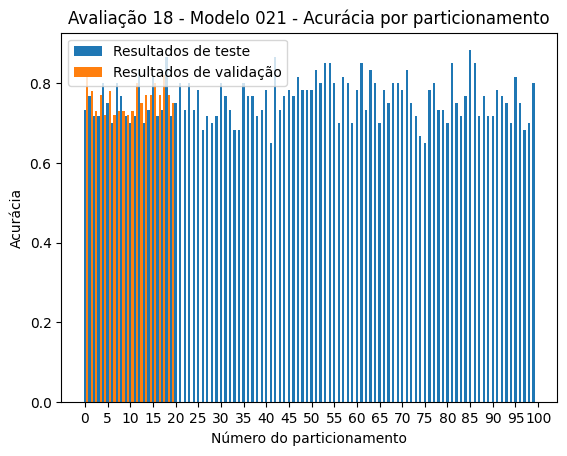
\includegraphics[scale=0.5]{images/grafico_barras_resultados_melhor_modelo.png}
    \label{fig:best_results_barplot}
  }
  \subfigure[Gráfico de caixa]{
    \centering
    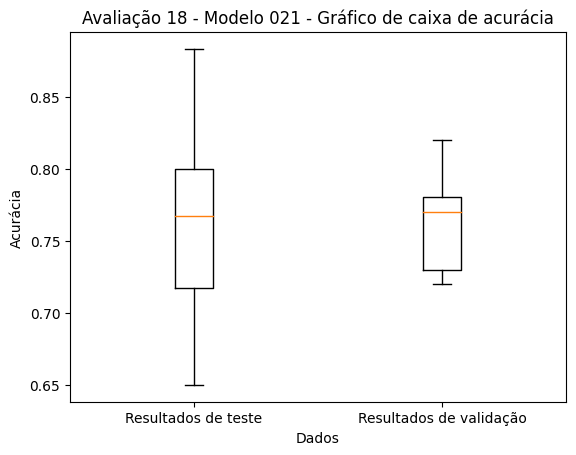
\includegraphics[scale=0.5]{images/grafico_caixa_resultados_melhor_modelo.png}
    \label{fig:best_results_boxplot}
  }
  \subfigure[Histograma]{
    \centering
    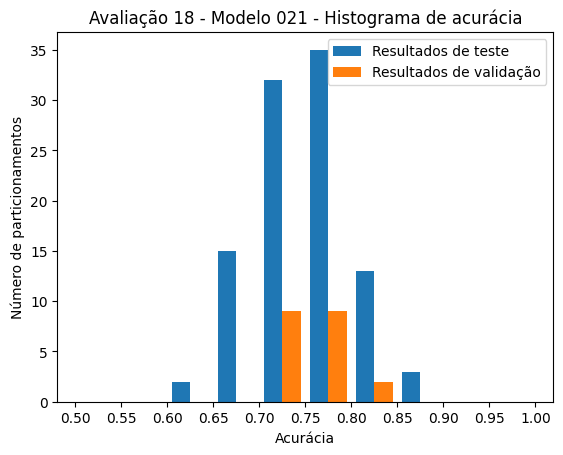
\includegraphics[scale=0.5]{images/histograma_resultados_melhor_modelo.png}
    \label{fig:best_results_histogram}
  }
	\caption{Gráficos de resultados para o melhor modelo do rankeamento.}
	\label{fig:best_results_plot}
\end{figure}

\section{Website}

O resultado a ser apresentado relativo ao website seria o website em si, o qual funcionou adequadamente, permitindo que um usuário criasse pacientes e requisitasse previsões de insuficiência cardíaca para estes, as quais foram processadas pelo \textit{backend} e tiveram seus resultados fornecidos. Porém, como não é possível apresentar todo o website e seu funcionamento neste documento, algumas páginas do website foram fornecidas com o intuito de ilustar a aplicação desenvolvida.

Na imagem \ref{fig:website_login_page} temos a página de login, que descreve o website ao usuário e permite que este realize login no website ou seja direcionado para a página de cadastro. Na imagem \ref{fig:website_home_page} temos a página principal do usuário, na qual os pacientes deste podem ser visualizados e gerenciados. Por fim, na imagem \ref{fig:website_patient_predictions_page} temos a página de previsões de um paciente, onde podemos visualizar as informações de um paciente e suas previsões realizadas e excluir previsões indesejadas.

\begin{figure}[ht!]
	\centering
  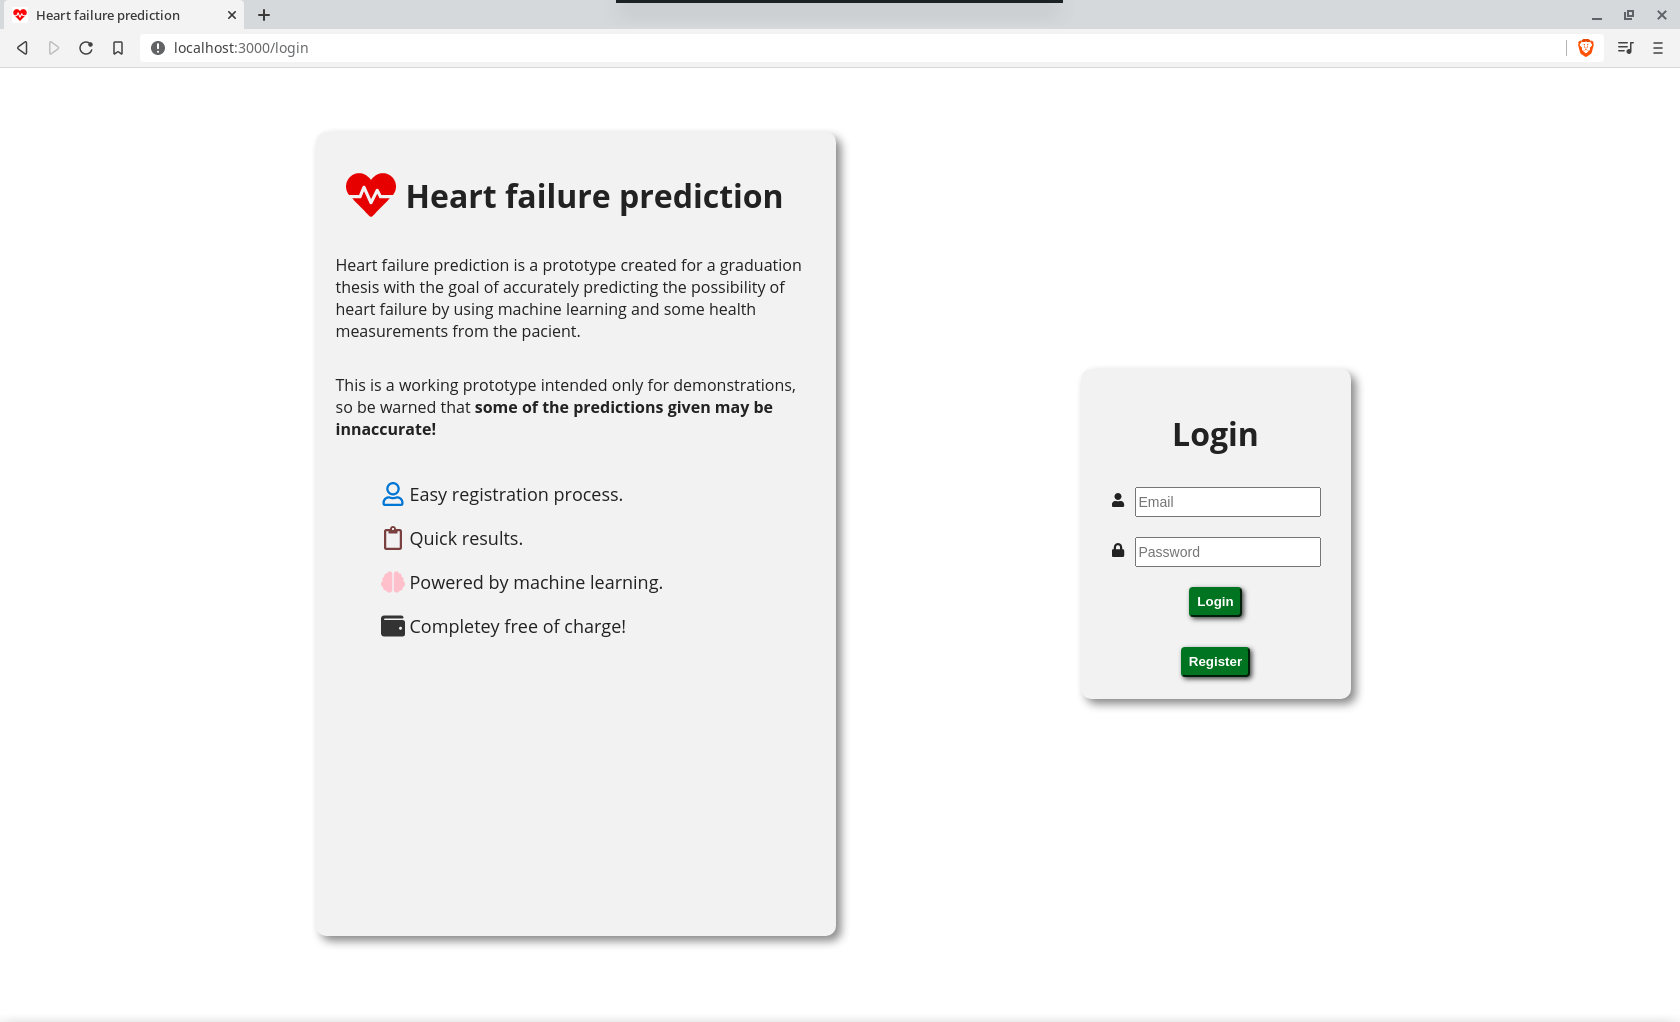
\includegraphics[scale=0.26]{images/website_pagina_login.png}
  \caption{Página de login do website}
  \label{fig:website_login_page}
\end{figure}

\begin{figure}[ht!]
  \centering
  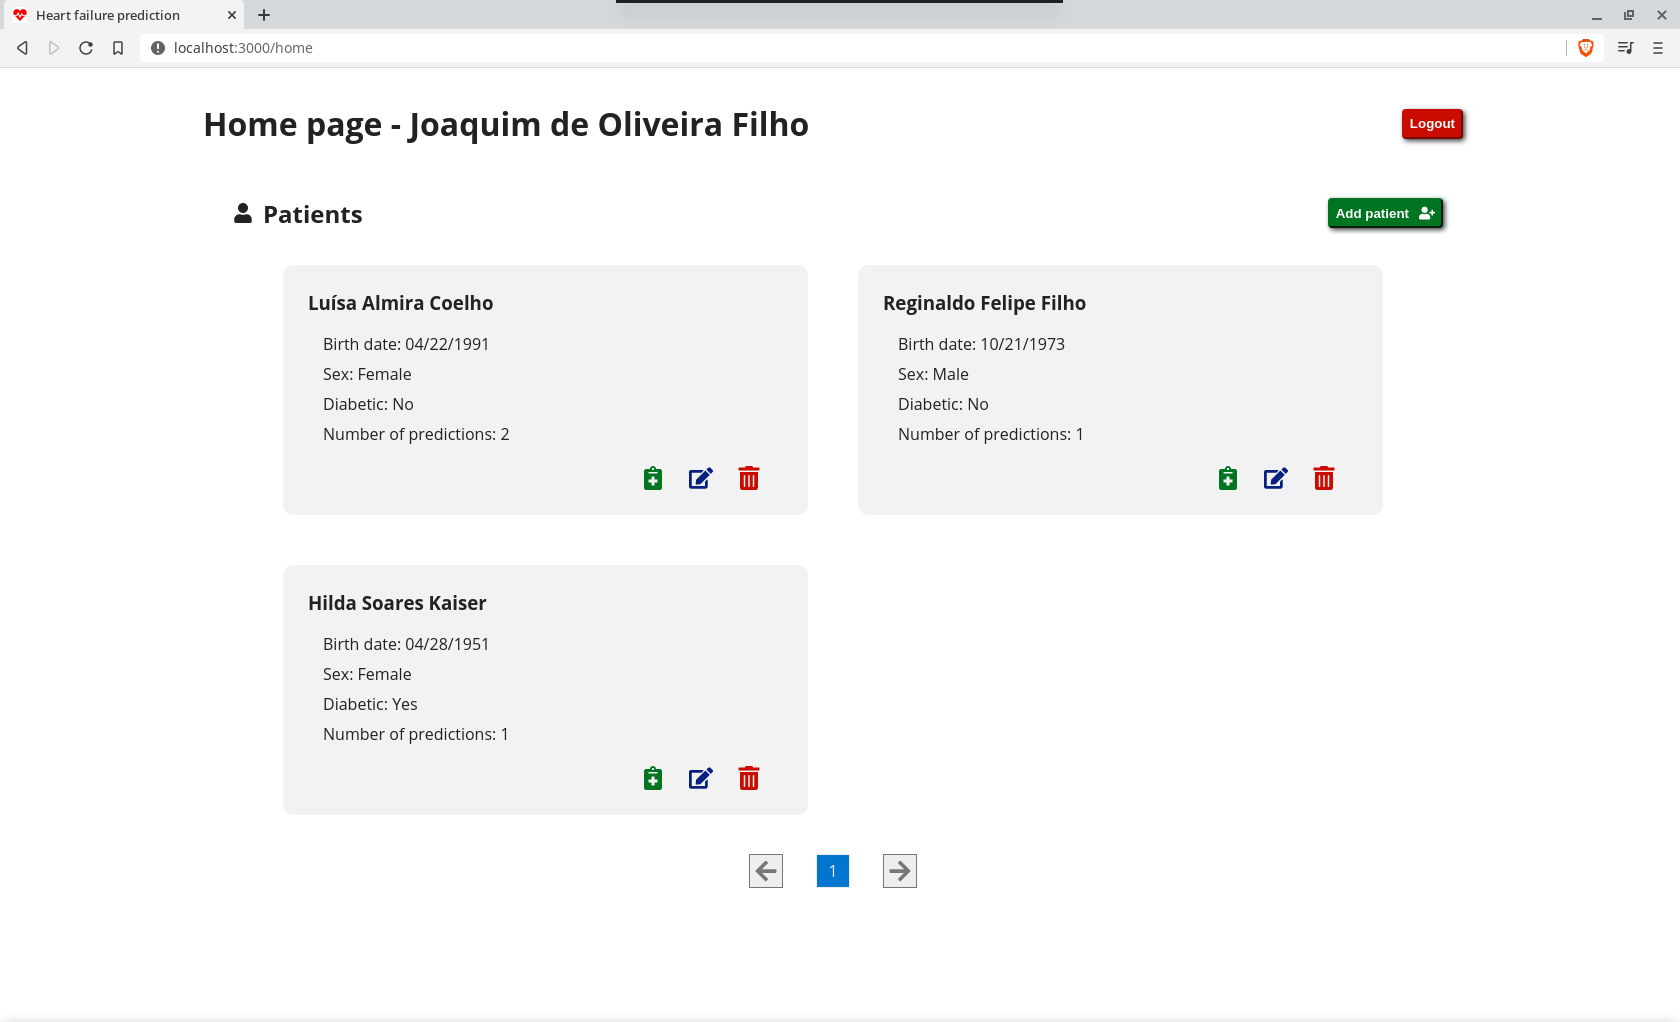
\includegraphics[scale=0.26]{images/website_pagina_home.png}
  \caption{Página principal do usuário do website}
  \label{fig:website_home_page}
\end{figure}

\begin{figure}[ht!]
  \centering
  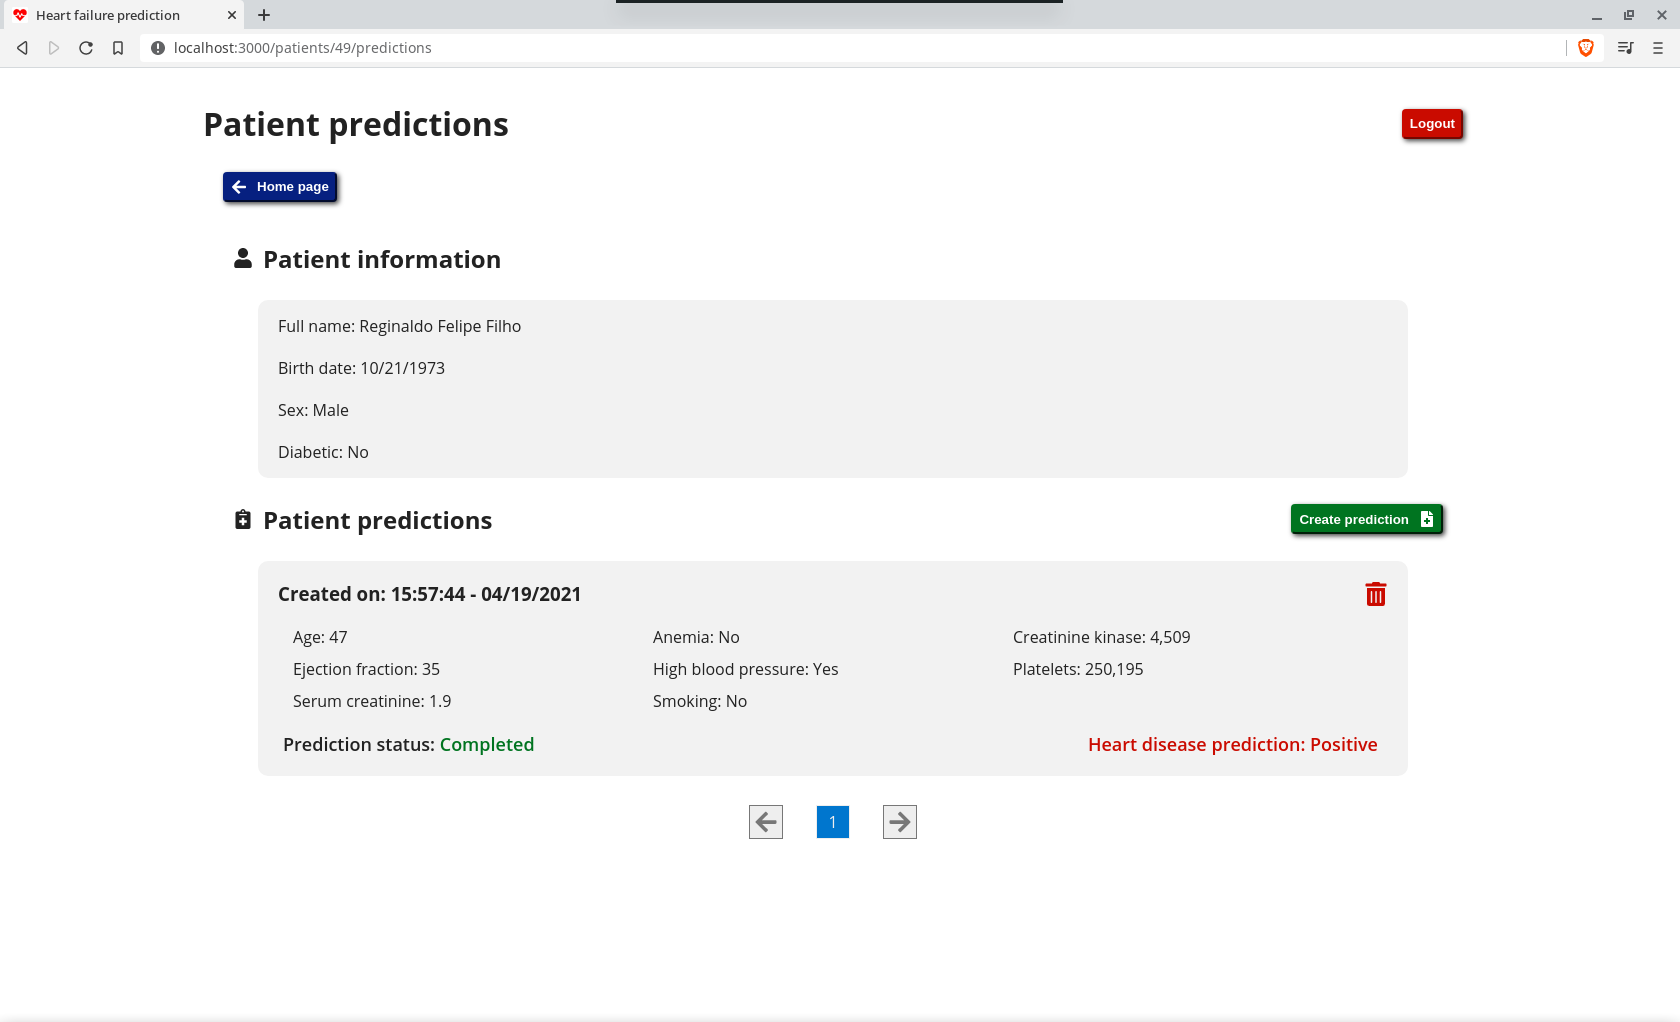
\includegraphics[scale=0.26]{images/website_pagina_previsoes_paciente.png}
  \caption{Página de previsões de um paciente do website}
  \label{fig:website_patient_predictions_page}
\end{figure}

Caso o leitor deseje explorar o funcionamento do website mais a fundo ou entender detalhes de sua implementação, o código fonte tanto do \textit{backend} como do \textit{frontend} pode ser encontrado no repositório do \textit{GitHub} deste trabalho\footnote{\url{https://github.com/AndreLaranjeira/ML-HeartFailure}}.

	\chapter{Futuras pesquisas} \label{chap:futuras_pesquisas}

Esse capítulo possui o intuito de abordar ideias para futuras pesquisas relacionadas a esse trabalho, incluindo suas motivações e impactos esperados.

\section{Utilização de dados de pacientes contemporâneos}

Este trabalho utilizou um conjunto de dados\cite{larxel_dataset} para realizar o treinamento dos modelos de aprendizado de máquina, mas não foi possível utilizar dados de pacientes contemporâneos para treinar os modelos de aprendizado ou para testar a acurácia do modelo empregado no website auxiliar. A utilização de dados de pacientes não cadastrados no conjunto de dados seria interessante tanto para mitigar algumas das limitações do conjunto de dados em questão, as quais são abordadas no capítulo \ref{chap:procedimento_adotado}, quanto para verificar a acurácia do modelo em um caso contemporâneo.

A obtenção dos dados em questão de um paciente qualquer não é necessariamente trabalhosa para um profissional médico, mas contém uma gama de implicações legais e éticas que devem ser discutidas com o paciente, o que poderia ser trabalhado em uma pesquisa futura. Espera-se que a utilização de dados de pacientes contemporâneos torne o aprendizado dos modelos mais robusto, aumentado a acurácia obtida para os subconjuntos de teste e tornando mais viável o uso do website em casos cotidianos.

\section{Avaliação de mais tipos de modelos de treinamento e variações de hiperparâmetros}

Este trabalho avaliou modelos de treinamento do tipo floresta aleatória e perceptron multicamada, utilizando 5346 combinações diferentes de hiperparâmetros para a realização de 30 avaliações envolvendo ambos os tipos de modelos conforme o método descrito no capítulo \ref{chap:procedimento_adotado}. Entretanto, ainda existem outros tipos de modelos de treinamento que foram mencionados no artigo científico de Chicco e Jurman\cite{chicco2020} que primeiramente estudou o conjunto de dados em questão e outras variações de hiperparâmetros para os tipos de modelos já avaliados neste trabalho.

O artigo em questão aponta os modelos do tipo árvore de decisão, \textit{extreme gradient boosting} e regressão linear como modelos que fornecem boas acurácias de previsão para o conjunto de dados em questão. E, para modelos do tipo floresta aleatória e perceptron multicamada, podemos citar, respectivamente, a exploração do hiperparâmetro de valor mínimo de decréscimo de impureza por divisão e redes neurais com 3 camadas escondidas ou que utilizem \textit{dropout} e \textit{kernels} de regularação \textit{simultaneamente} como variações interessantes de hiperparâmetros que ainda podem ser exploradas. Com a utilização de um número maior de tipos de modelos de treinamento e de mais variações de hiperparâmetros para estes modelos de treinamento, podemos, possivelmente, melhorar os resultados de acurácia obtidos na previsão de insuficiência cardíaca.

\section{Criação de um aplicativo móvel para o projeto}

Como mencionado no capítulo \ref{chap:procedimento_adotado}, o website auxiliar foi desenvolvido com um \textit{backend} sendo uma \textit{API}, de forma que um novo \textit{frontend} pode ser facilmente desenvolvido para interagir com o banco de dados aproveitando o \textit{backend} existente. Uma sugestão de \textit{frontend} a ser desenvolvido é um aplicativo móvel que possa ser utilizado em \textit{smartphones}.

O uso de \textit{smartphones} nos dias atuais é uma alternativa extremamente popular ao uso de computadores e \textit{notebooks} por sua versatilidade, facilidade de uso e maiores opções de quando e onde um serviço pode ser utilizado. Dessa forma, seria benéfico ao usuário do website auxiliar poder utilizar o serviço de previsão de insuficiência cardíaca por meio de um aplicativo em seu \textit{smartphone}.

	\chapter{Conclusão} \label{chap:conclusao}

Insira sua conclusão aqui.


	%\bibliographystyle{bibliography/abnt-num} % estilo bibliográfico ABNT numérico
	%\bibliographystyle{bibliography/abnt-alf} % estilo bibliográfico ABNT alfabético
	\bibliographystyle{bibliography/sbc}  % estilo bibliográfico da Sociedade Brasileira de Computação (SBC)

	%\renewcommand{\bibname}{REFERÊNCIAS BIBLIOGRÁFICAS} %Define o Caption da seção de bibliografia
	%\addcontentsline{toc}{chapter}{REFERÊNCIAS BIBLIOGRÁFICAS}

	%não pode ter espaço entre os nomes dos arquivos bib
	\bibliography{bibliography/referencias}

  % Seção comentada porque não foi utilizada.
	% \include{sections/apendice}
\end{document}
